% Options for packages loaded elsewhere
\PassOptionsToPackage{unicode}{hyperref}
\PassOptionsToPackage{hyphens}{url}
\PassOptionsToPackage{dvipsnames,svgnames,x11names}{xcolor}
%
\documentclass[
  letterpaper,
  12pt,
  oneside,
  spanish,
  doublespacing,
  headsepline]{MastersDoctoralThesis}

\usepackage{amsmath,amssymb}
\usepackage{lmodern}
\usepackage{iftex}
\ifPDFTeX
  \usepackage[T1]{fontenc}
  \usepackage[utf8]{inputenc}
  \usepackage{textcomp} % provide euro and other symbols
\else % if luatex or xetex
  \usepackage{unicode-math}
  \defaultfontfeatures{Scale=MatchLowercase}
  \defaultfontfeatures[\rmfamily]{Ligatures=TeX,Scale=1}
\fi
% Use upquote if available, for straight quotes in verbatim environments
\IfFileExists{upquote.sty}{\usepackage{upquote}}{}
\IfFileExists{microtype.sty}{% use microtype if available
  \usepackage[]{microtype}
  \UseMicrotypeSet[protrusion]{basicmath} % disable protrusion for tt fonts
}{}
\makeatletter
\@ifundefined{KOMAClassName}{% if non-KOMA class
  \IfFileExists{parskip.sty}{%
    \usepackage{parskip}
  }{% else
    \setlength{\parindent}{0pt}
    \setlength{\parskip}{6pt plus 2pt minus 1pt}}
}{% if KOMA class
  \KOMAoptions{parskip=half}}
\makeatother
\usepackage{xcolor}
\usepackage[paper=a4paper,inner=2.5cm,outer=2.5cm,top=2.5cm,bottom=2.5cm]{geometry}
\usepackage[normalem]{ulem}
\setlength{\emergencystretch}{3em} % prevent overfull lines
\setcounter{secnumdepth}{5}
% Make \paragraph and \subparagraph free-standing
\ifx\paragraph\undefined\else
  \let\oldparagraph\paragraph
  \renewcommand{\paragraph}[1]{\oldparagraph{#1}\mbox{}}
\fi
\ifx\subparagraph\undefined\else
  \let\oldsubparagraph\subparagraph
  \renewcommand{\subparagraph}[1]{\oldsubparagraph{#1}\mbox{}}
\fi

\usepackage{color}
\usepackage{fancyvrb}
\newcommand{\VerbBar}{|}
\newcommand{\VERB}{\Verb[commandchars=\\\{\}]}
\DefineVerbatimEnvironment{Highlighting}{Verbatim}{commandchars=\\\{\}}
% Add ',fontsize=\small' for more characters per line
\usepackage{framed}
\definecolor{shadecolor}{RGB}{241,243,245}
\newenvironment{Shaded}{\begin{snugshade}}{\end{snugshade}}
\newcommand{\AlertTok}[1]{\textcolor[rgb]{0.68,0.00,0.00}{#1}}
\newcommand{\AnnotationTok}[1]{\textcolor[rgb]{0.37,0.37,0.37}{#1}}
\newcommand{\AttributeTok}[1]{\textcolor[rgb]{0.40,0.45,0.13}{#1}}
\newcommand{\BaseNTok}[1]{\textcolor[rgb]{0.68,0.00,0.00}{#1}}
\newcommand{\BuiltInTok}[1]{\textcolor[rgb]{0.00,0.23,0.31}{#1}}
\newcommand{\CharTok}[1]{\textcolor[rgb]{0.13,0.47,0.30}{#1}}
\newcommand{\CommentTok}[1]{\textcolor[rgb]{0.37,0.37,0.37}{#1}}
\newcommand{\CommentVarTok}[1]{\textcolor[rgb]{0.37,0.37,0.37}{\textit{#1}}}
\newcommand{\ConstantTok}[1]{\textcolor[rgb]{0.56,0.35,0.01}{#1}}
\newcommand{\ControlFlowTok}[1]{\textcolor[rgb]{0.00,0.23,0.31}{#1}}
\newcommand{\DataTypeTok}[1]{\textcolor[rgb]{0.68,0.00,0.00}{#1}}
\newcommand{\DecValTok}[1]{\textcolor[rgb]{0.68,0.00,0.00}{#1}}
\newcommand{\DocumentationTok}[1]{\textcolor[rgb]{0.37,0.37,0.37}{\textit{#1}}}
\newcommand{\ErrorTok}[1]{\textcolor[rgb]{0.68,0.00,0.00}{#1}}
\newcommand{\ExtensionTok}[1]{\textcolor[rgb]{0.00,0.23,0.31}{#1}}
\newcommand{\FloatTok}[1]{\textcolor[rgb]{0.68,0.00,0.00}{#1}}
\newcommand{\FunctionTok}[1]{\textcolor[rgb]{0.28,0.35,0.67}{#1}}
\newcommand{\ImportTok}[1]{\textcolor[rgb]{0.00,0.46,0.62}{#1}}
\newcommand{\InformationTok}[1]{\textcolor[rgb]{0.37,0.37,0.37}{#1}}
\newcommand{\KeywordTok}[1]{\textcolor[rgb]{0.00,0.23,0.31}{#1}}
\newcommand{\NormalTok}[1]{\textcolor[rgb]{0.00,0.23,0.31}{#1}}
\newcommand{\OperatorTok}[1]{\textcolor[rgb]{0.37,0.37,0.37}{#1}}
\newcommand{\OtherTok}[1]{\textcolor[rgb]{0.00,0.23,0.31}{#1}}
\newcommand{\PreprocessorTok}[1]{\textcolor[rgb]{0.68,0.00,0.00}{#1}}
\newcommand{\RegionMarkerTok}[1]{\textcolor[rgb]{0.00,0.23,0.31}{#1}}
\newcommand{\SpecialCharTok}[1]{\textcolor[rgb]{0.37,0.37,0.37}{#1}}
\newcommand{\SpecialStringTok}[1]{\textcolor[rgb]{0.13,0.47,0.30}{#1}}
\newcommand{\StringTok}[1]{\textcolor[rgb]{0.13,0.47,0.30}{#1}}
\newcommand{\VariableTok}[1]{\textcolor[rgb]{0.07,0.07,0.07}{#1}}
\newcommand{\VerbatimStringTok}[1]{\textcolor[rgb]{0.13,0.47,0.30}{#1}}
\newcommand{\WarningTok}[1]{\textcolor[rgb]{0.37,0.37,0.37}{\textit{#1}}}

\providecommand{\tightlist}{%
  \setlength{\itemsep}{0pt}\setlength{\parskip}{0pt}}\usepackage{longtable,booktabs,array}
\usepackage{calc} % for calculating minipage widths
% Correct order of tables after \paragraph or \subparagraph
\usepackage{etoolbox}
\makeatletter
\patchcmd\longtable{\par}{\if@noskipsec\mbox{}\fi\par}{}{}
\makeatother
% Allow footnotes in longtable head/foot
\IfFileExists{footnotehyper.sty}{\usepackage{footnotehyper}}{\usepackage{footnote}}
\makesavenoteenv{longtable}
\usepackage{graphicx}
\makeatletter
\def\maxwidth{\ifdim\Gin@nat@width>\linewidth\linewidth\else\Gin@nat@width\fi}
\def\maxheight{\ifdim\Gin@nat@height>\textheight\textheight\else\Gin@nat@height\fi}
\makeatother
% Scale images if necessary, so that they will not overflow the page
% margins by default, and it is still possible to overwrite the defaults
% using explicit options in \includegraphics[width, height, ...]{}
\setkeys{Gin}{width=\maxwidth,height=\maxheight,keepaspectratio}
% Set default figure placement to htbp
\makeatletter
\def\fps@figure{htbp}
\makeatother
\newlength{\cslhangindent}
\setlength{\cslhangindent}{1.5em}
\newlength{\csllabelwidth}
\setlength{\csllabelwidth}{3em}
\newlength{\cslentryspacingunit} % times entry-spacing
\setlength{\cslentryspacingunit}{\parskip}
\newenvironment{CSLReferences}[2] % #1 hanging-ident, #2 entry spacing
 {% don't indent paragraphs
  \setlength{\parindent}{0pt}
  % turn on hanging indent if param 1 is 1
  \ifodd #1
  \let\oldpar\par
  \def\par{\hangindent=\cslhangindent\oldpar}
  \fi
  % set entry spacing
  \setlength{\parskip}{#2\cslentryspacingunit}
 }%
 {}
\usepackage{calc}
\newcommand{\CSLBlock}[1]{#1\hfill\break}
\newcommand{\CSLLeftMargin}[1]{\parbox[t]{\csllabelwidth}{#1}}
\newcommand{\CSLRightInline}[1]{\parbox[t]{\linewidth - \csllabelwidth}{#1}\break}
\newcommand{\CSLIndent}[1]{\hspace{\cslhangindent}#1}

\usepackage[utf8]{inputenc} % Required for inputting international characters
\usepackage[T1]{fontenc} % Output font encoding for international characters

% \usepackage{mathpazo} % Use the Palatino font by default
\usepackage{fontspec}
\setmainfont{Arial}

\usepackage[backend=bibtex, style=authoryear, natbib=true]{biblatex}
% \RequirePackage{bibspacing}
% \setlength\bibitemsep{\baselineskip} % un enter entre cada fuente

% \newlength{\bibitemsep}\setlength{\bibitemsep}{.2\baselineskip plus .05\baselineskip minus .05\baselineskip}
% \newlength{\bibparskip}\setlength{\bibparskip}{0pt}
% \let\oldthebibliography\thebibliography
% \renewcommand\thebibliography[1]{%
%   \oldthebibliography{#1}%
%   \setlength{\parskip}{\bibitemsep}%
%   \setlength{\itemsep}{\bibparskip}%
% }

% Use the bibtex backend with the authoryear citation style (which resembles APA)

\usepackage[autostyle=true]{csquotes} % Required to generate language-dependent quotes in the bibliography

%----------------------------------------------------------------------------------------
%	MARGINS
%----------------------------------------------------------------------------------------

\geometry{ % ?
	headheight=4ex,
	includehead,
	includefoot
}

\raggedbottom
% \setlength\bibitemsep{\baselineskip}
% \printbibliography
\AtBeginDocument{
\hypersetup{pdftitle=\ttitle} % Set the PDF's title to your title
\hypersetup{pdfauthor=\authorname} % Set the PDF's author to your name
\hypersetup{pdfkeywords=\keywordnames} % Set the PDF's keywords to your keywords
}
\usepackage{booktabs}
\usepackage{longtable}
\usepackage{array}
\usepackage{multirow}
\usepackage{wrapfig}
\usepackage{float}
\usepackage{colortbl}
\usepackage{pdflscape}
\usepackage{tabu}
\usepackage{threeparttable}
\usepackage{threeparttablex}
\usepackage[normalem]{ulem}
\usepackage{makecell}
\usepackage{xcolor}
\makeatletter
\makeatother
\makeatletter
\@ifpackageloaded{bookmark}{}{\usepackage{bookmark}}
\makeatother
\makeatletter
\@ifpackageloaded{caption}{}{\usepackage{caption}}
\AtBeginDocument{%
\ifdefined\contentsname
  \renewcommand*\contentsname{Indice de contenidos}
\else
  \newcommand\contentsname{Indice de contenidos}
\fi
\ifdefined\listfigurename
  \renewcommand*\listfigurename{Listado de Figuras}
\else
  \newcommand\listfigurename{Listado de Figuras}
\fi
\ifdefined\listtablename
  \renewcommand*\listtablename{Listado de Tablas}
\else
  \newcommand\listtablename{Listado de Tablas}
\fi
\ifdefined\figurename
  \renewcommand*\figurename{Figura}
\else
  \newcommand\figurename{Figura}
\fi
\ifdefined\tablename
  \renewcommand*\tablename{Tabla}
\else
  \newcommand\tablename{Tabla}
\fi
}
\@ifpackageloaded{float}{}{\usepackage{float}}
\floatstyle{ruled}
\@ifundefined{c@chapter}{\newfloat{codelisting}{h}{lop}}{\newfloat{codelisting}{h}{lop}[chapter]}
\floatname{codelisting}{Listado}
\newcommand*\listoflistings{\listof{codelisting}{Listado de Listatdos}}
\makeatother
\makeatletter
\@ifpackageloaded{caption}{}{\usepackage{caption}}
\@ifpackageloaded{subcaption}{}{\usepackage{subcaption}}
\makeatother
\makeatletter
\@ifpackageloaded{tcolorbox}{}{\usepackage[many]{tcolorbox}}
\makeatother
\makeatletter
\@ifundefined{shadecolor}{\definecolor{shadecolor}{rgb}{.97, .97, .97}}
\makeatother
\makeatletter
\makeatother
\ifLuaTeX
\usepackage[bidi=basic]{babel}
\else
\usepackage[bidi=default]{babel}
\fi
\babelprovide[main,import]{spanish}
% get rid of language-specific shorthands (see #6817):
\let\LanguageShortHands\languageshorthands
\def\languageshorthands#1{}
\ifLuaTeX
  \usepackage{selnolig}  % disable illegal ligatures
\fi
\IfFileExists{bookmark.sty}{\usepackage{bookmark}}{\usepackage{hyperref}}
\IfFileExists{xurl.sty}{\usepackage{xurl}}{} % add URL line breaks if available
\urlstyle{same} % disable monospaced font for URLs
\hypersetup{
  pdftitle={El efecto de la pandemia del COVID-19 en las condiciones de vida de las familias de trabajadores del sector informal en el Perú urbano},
  pdfauthor={Sotelo Galindo, Santiago Salvador},
  pdflang={es},
  colorlinks=true,
  linkcolor={black},
  filecolor={Maroon},
  citecolor={blue},
  urlcolor={blue},
  pdfcreator={LaTeX via pandoc}}

\thesistitle{El efecto de la pandemia del COVID-19 en las condiciones de
vida de las familias de trabajadores del sector informal en el Perú
urbano} % Your thesis title, this is used in the title and abstract, print it elsewhere with \ttitle

\supervisor{Sulmont,
David} % Your supervisor's name, this is used in the title page, print it elsewhere with \supname

\examiner{} % Your examiner's name, this is not currently used anywhere in the template, print it elsewhere with \examname

\degree{Licenciado en
Sociología} % Your degree name, this is used in the title page and abstract, print it elsewhere with \degreename

\author{Sotelo Galindo, Santiago
Salvador} % Your name, this is used in the title page and abstract, print it elsewhere with \authorname

\addresses{} % Your address, this is not currently used anywhere in the template, print it elsewhere with \addressname

\subject{} % Your subject area, this is not currently used anywhere in the template, print it elsewhere with \subjectname

\keywords{capital social,
desigualdad} % Your keywords, this is used in the title page and abstract, print it elsewhere with \keywordname

\city{Lima} % Your city's name, this is used in the title page and abstract, print it elsewhere with \cityname

\dateyear{2022} % Your year, this is used in the title page and abstract, print it elsewhere with \dateyearname

\university{} % Your university's name, this is used in the title page and abstract, print it elsewhere with \univname

\department{Department of
Mathematics} % Your department's name, this is used in the title page and abstract, print it elsewhere with \deptname

\group{Informatics
Program} % Your research group's name and URL, this is used in the title page, print it elsewhere with \groupname

\faculty{Facultad de Ciencias
Sociales} % Your faculty's name and URL, this is used in the title page and abstract, print it elsewhere with \facname

\setcounter{tocdepth}{1} % The depth to which the document sections are printed to the table of contents
\begin{document}
\pagestyle{empty} % Default to the plain heading style until the thesis style is called for the body content
\pagenumbering{gobble} % funcionó para quitarle la numeración de página
%----------------------------------------------------------------------------------------
%	TITLE PAGE
%----------------------------------------------------------------------------------------

\begin{titlepage}
\DraftwatermarkOptions{stamp=false} % quitarle la marca de agua a la primera página
\begin{center}

\vspace*{.06\textheight}
{\MakeUppercase{\textbf{PONTIFICIA UNIVERSIDAD \\ CATÓLICA DEL PERÚ}}\par}\vspace{0.25cm} % University name
\MakeUppercase{\textbf{\facname}}\vspace{0.5cm} % Thesis type


\includegraphics[width=6cm]{pucp_escudo}\vspace{0.5cm}

{\textbf{\ttitle}\par}\vspace{0.4cm} % Thesis title

{Tesis para obtener el título profesional de \degreename}{ presentado por:}\\[0.3cm] % University requirement text

\authorname

{Asesor(es):}\\[0.4cm]
%
\href{http://www.google.com}{\supname} % Supervisor name - remove the \href bracket to remove the link


{\cityname}{, }{\dateyearname}

\vfill
\end{center}
\end{titlepage}

%----------------------------------------------------------------------------------------
%	DEDICATION
%----------------------------------------------------------------------------------------

\dedicatory{Para Elsa} 
\newpage


%----------------------------------------------------------------------------------------
%	ACKNOWLEDGEMENTS
%----------------------------------------------------------------------------------------

\begin{acknowledgements}
\begin{singlespace}
\addchaptertocentry{\acknowledgementname} % Add the acknowledgements to the table of contents
Integer id risus vel lorem laoreet commodo lobortis quis purus. Cras cursus leo vel dui laoreet pulvinar. Nunc tincidunt metus et ante fermentum lacinia. Proin quam magna, tristique ut viverra at, dapibus eget elit. Quisque eu leo id nisi semper laoreet at ac nulla. Fusce volutpat, metus sed dictum mattis, nisl elit dapibus velit, non porttitor urna urna vel diam. Praesent tortor nulla, rutrum ac magna a, tempor sagittis enim. Praesent pharetra ipsum libero, eu malesuada libero blandit ut. Sed sed venenatis ligula, nec convallis turpis. Nulla iaculis felis eros, eget pharetra lorem cursus quis. Nunc iaculis lobortis magna at malesuada. Nullam elementum elit at urna congue aliquam.
\end{singlespace}
\end{acknowledgements}


%----------------------------------------------------------------------------------------
%	ABSTRACT PAGE
%----------------------------------------------------------------------------------------

\begin{abstract}
\begin{singlespace}
\addchaptertocentry{\abstractname} % Add the abstract to the table of contents
{Lorem ipsum dolor sit amet, consectetur adipiscing elit. Aliquam quis
accumsan ante. Quisque lorem metus, varius id urna eget, lacinia dapibus
sem. Etiam laoreet, quam ac mollis congue, arcu leo dictum neque, nec
euismod sem enim luctus odio. Donec condimentum tortor sit amet mollis
volutpat.}\vspace{0.3cm}

{Palabras clave: }{\keywordnames}% palabras clave
\end{singlespace}
\end{abstract}


% 

\tableofcontents % Prints the main table of contents

\listoffigures % Prints the list of figures

\listoftables % Prints the list of tables

%----------------------------------------------------------------------------------------
%	ABBREVIATIONS
%----------------------------------------------------------------------------------------

\begin{abbreviations}{ll} % Include a list of abbreviations (a table of two columns)

\textbf{LAH} & \textbf{L}ist \textbf{A}bbreviations \textbf{H}ere\\
\textbf{WSF} & \textbf{W}hat (it) \textbf{S}tands \textbf{F}or\\

\end{abbreviations}



%----------------------------------------------------------------------------------------
%	PHYSICAL CONSTANTS/OTHER DEFINITIONS
%----------------------------------------------------------------------------------------

\begin{constants}{lr@{${}={}$}l} % The list of physical constants is a three column table

% The \SI{}{} command is provided by the siunitx package, see its documentation for instructions on how to use it

Speed of Light & $c_{0}$ & \SI{2.99792458e8}{\meter\per\second} (exact)\\
%Constant Name & $Symbol$ & $Constant Value$ with units\\

\end{constants}




%----------------------------------------------------------------------------------------
%	SYMBOLS
%----------------------------------------------------------------------------------------

\begin{symbols}{lll} % Include a list of Symbols (a three column table)

$a$ & distance & m \\
$P$ & power & W (J s$^1$) \\
%Symbol & Name & Unit \\

\addlinespace % Gap to separate the Roman symbols from the Greek

$\omega$ & angular frequency & rad \\

\end{symbols}


%----------------------------------------------------------------------------------------
%	THESIS CONTENT - CHAPTERS
%----------------------------------------------------------------------------------------

\mainmatter

\pagestyle{thesis} % Return the page headers back to the "thesis" style

% Define some commands to keep the formatting separated from the content 
\newcommand{\keyword}[1]{\textbf{#1}}
\newcommand{\tabhead}[1]{\textbf{#1}}
\newcommand{\code}[1]{\texttt{#1}}
\newcommand{\file}[1]{\texttt{\bfseries#1}}
\newcommand{\option}[1]{\texttt{\itshape#1}}

\ifdefined\Shaded\renewenvironment{Shaded}{\begin{tcolorbox}[borderline west={3pt}{0pt}{shadecolor}, interior hidden, breakable, frame hidden, sharp corners, boxrule=0pt, enhanced]}{\end{tcolorbox}}\fi

\bookmarksetup{startatroot}

\hypertarget{sec-Chapter1}{%
\chapter{Chapter 1 Title}\label{sec-Chapter1}}

\hypertarget{welcome-and-thank-you}{%
\section{Welcome and Thank You}\label{welcome-and-thank-you}}

Welcome to this \LaTeX{} Thesis Template, using the \LaTeX{} typesetting
system and \href{quarto.org}{Quarto} and based on the \LaTeX{} thesis
template MastersDoctoralThesis version 2.0 downloaded from
\href{http://www.LaTeXTemplates.com}{LaTeXTemplates}. The class was
authored by Vel (vel@latextemplates.com) and Johannes Böttcher based on
a style file by Steve R. Gunn from the University of Southampton (UK),
department of Electronics and Computer Science.

\hypertarget{a-short-math-guide-for}{%
\section{\texorpdfstring{A Short Math Guide for
\LaTeX{}}{A Short Math Guide for }}\label{a-short-math-guide-for}}

If you are writing a technical or mathematical thesis, then you may want
to read the document by the AMS (American Mathematical Society) called,
\enquote{A Short Math Guide for \LaTeX{}}. It can be found online at
\href{http://www.ams.org/tex/amslatex.html}{AMS} under the
\enquote{Additional Documentation} section towards the bottom of the
page.

\hypertarget{common-math-symbols}{%
\subsection{\texorpdfstring{Common \LaTeX{} Math
Symbols}{Common  Math Symbols}}\label{common-math-symbols}}

There are a multitude of mathematical symbols available for \LaTeX{} and
it would take a great effort to learn the commands for them all. The
most common ones you are likely to use are shown on
\href{http://www.sunilpatel.co.uk/latex-type/latex-math-symbols/}{this
page}.

You can use this page as a reference or crib sheet, the symbols are
rendered as large, high quality images so you can quickly find the
\LaTeX{} command for the symbol you need.

\hypertarget{about-this-template}{%
\section{About this Template}\label{about-this-template}}

This \LaTeX{} Thesis Template is originally based and created around a
\LaTeX{} style file created by Steve R. Gunn from the University of
Southampton (UK), department of Electronics and Computer Science. You
can find his original thesis style file at his site, here:
http://www.ecs.soton.ac.uk/\textasciitilde srg/softwaretools/document/templates/.

Steve's \texttt{ecsthesis.cls} was then taken by Sunil Patel who
modified it by creating a skeleton framework and folder structure to
place the thesis files in. The resulting template can be found on
Sunil's site here: http://www.sunilpatel.co.uk/thesis-template.

Sunil's template was made available through
\href{http://www.LaTeXTemplates.com}{LaTeXTemplates} where it was
modified many times based on user requests and questions. Version 2.0
and onwards of this template represents a major modification to Sunil's
template and is, in fact, hardly recognisable. The work to make version
2.0 possible was carried out by Vel (vel@latextemplates.com) and
Johannes Böttcher.

\hypertarget{what-this-template-includes}{%
\section{What this Template
Includes}\label{what-this-template-includes}}

\hypertarget{folders}{%
\subsection{Folders}\label{folders}}

\begin{itemize}
\item
  Appendices -- this is the folder where you put the appendices. Each
  appendix should go into its own separate qmd file. An example and
  template are included in the directory.
\item
  Chapters -- this is the folder where you put the thesis chapters. Each
  chapter should go in its own separate qmd file.
\item
  Figures -- this folder contains static figures for the thesis,
  i.e.~figures that are not generated by code in the chapters.
\end{itemize}

\hypertarget{files}{%
\subsection{Files}\label{files}}

\begin{itemize}
\item
  example.bib -- this is file that contains all the bibliographic
  information and references that you will be citing in the thesis for
  use with BibTeX. You can write it manually, but there are reference
  manager programs available that will create and manage it for you.
  Zotero is popular and integrates with RStudio IDE if you use that.
\item
  MastersDoctoralThesis.cls -- this is the class file that tells
  \LaTeX{} how to format the thesis.
\item
  pdf in docs folder -- this is your typeset thesis.
\item
  Frontmater folder -- this has the files for the various front matter
  elements.
\end{itemize}

\hypertarget{filling-in-your-information}{%
\section{Filling in Your
Information}\label{filling-in-your-information}}

Most of the personal information is found on in the
\texttt{\_quarto.yml} file.

\begin{itemize}
\tightlist
\item
  author -- you; optionally add url
\item
  supervisor -- your supervisor; optionally add url.
\item
  university -- your university
\item
  department -- your department
\item
  faculty -- faculty name
\item
  group -- research group name (optional)
\item
  abstract
\end{itemize}

\hypertarget{the-texbefore-body.tex-file-explained}{%
\section{\texorpdfstring{The \texttt{tex\textbackslash{}before-body.tex}
File
Explained}{The tex\textbackslash before-body.tex File Explained}}\label{the-texbefore-body.tex-file-explained}}

The \texttt{tex\textbackslash{}before-body.tex} file contains the
structure of the thesis and is a mix of Pandoc template and \LaTeX{}
code. The bits that look like \texttt{\$book.university\$} say are
Pandoc and are referencing variables in the \texttt{\_quarto.yml} file.
Knowing that, you should be able to figure out what is happening.

There are plenty of written comments that explain what pages, sections
and formatting the \LaTeX{} code is creating. Each major document
element is divided into commented blocks with titles in all capitals to
make it obvious what the following bit of code is doing. Initially there
seems to be a lot of \LaTeX{} code, but this is all formatting, and it
has all been taken care of so you don't have to do it.

Many of the sections have \texttt{\$if(...)\$} so that the section is
only included if you included information for that in
\texttt{\_quarto.yml}.

In the \texttt{\_quarto.yml}, \texttt{pdf:\ toc:\ false} is used so that
Quarto/Pandoc doesn't add a table of contents. This template puts the
table of contents before the abbreviations and symbols pages and
Quarto/Pandoc doesn't let us control where it puts the table of
contents. So we have to add the TOC manually for pdf and pass in
\texttt{toc:\ false}.

The list of figures and tables are all taken care of for you and do not
need to be manually created or edited. The next set of pages are more
likely to be optional and can be deleted since they are for a more
technical thesis: insert a list of abbreviations you have used in the
thesis, then a list of the physical constants and numbers you refer to
and finally, a list of mathematical symbols used in any formulae. Making
the effort to fill these tables means the reader has a one-stop place to
refer to instead of searching the internet and references to try and
find out what you meant by certain abbreviations or symbols.

The list of symbols is split into the Roman and Greek alphabets. Whereas
the abbreviations and symbols ought to be listed in alphabetical order
(and this is \textbf{not} done automatically for you) the list of
physical constants should be grouped into similar themes.

The next page contains a one line dedication. Who will you dedicate your
thesis to?

\hypertarget{adding-your-chapters-and-appendices}{%
\section{Adding Your Chapters and
Appendices}\label{adding-your-chapters-and-appendices}}

Add your chapters and appendices to \texttt{\_quarto.yml}. Note that the
spacing is important as is the leading \texttt{-}.

\hypertarget{bibliography-and-citations}{%
\section{Bibliography and Citations}\label{bibliography-and-citations}}

Citations will be added and formatted automatically for you.

If you use the RStudio IDE, then you can link Zotero to RStudio and
Quarto will find your citations for you when you enter \texttt{@}. This
is in the visual editor mode. Make sure to search for videos on how to
do this as using Zotero libraries will make your citation and
bibliography management much much easier.

In the text use \texttt{@smith2000} to produce Smith (2000) add use
\texttt{{[}@smith2000,\ @jones1999{]}} to produce (Smith 2000; Jones
1999). See the natbib cheatsheet for how to do other types of formatting
for your in text citations. The bibliography style
(\texttt{classoption:\ "authoryear"}) is used for the bibliography and
is a fully featured style that will even include links to where the
referenced paper can be found online.

Acá las referencias reales de Hawthorn et~al. (2001), Wieman \& Hollberg
(1991), Arnold et~al. (1998).

\hypertarget{a-note-on-bibtex}{%
\subsubsection{A Note on bibtex}\label{a-note-on-bibtex}}

The bibtex backend used in the template by default does not correctly
handle unicode character encoding (i.e.~``international'' characters).
You may see a warning about this in the compilation log and, if your
references contain unicode characters, they may not show up correctly or
at all. One solution to this is to use the biber backend instead of the
outdated bibtex backend. This is done by finding this in
\texttt{tex/in-header.tex}: \texttt{backend=bibtex} and changing it to
\texttt{backend=biber}. Google a bit to find information on this.

\hypertarget{sec-ThesisConventions}{%
\section{Thesis Features and Conventions}\label{sec-ThesisConventions}}

To get the best out of this template, there are a few conventions that
you may want to follow.

\hypertarget{printing-format}{%
\subsection{Printing Format}\label{printing-format}}

This thesis template is designed for double sided printing (i.e.~content
on the front and back of pages) as most theses are printed and bound
this way. Switching to one sided printing is as simple as adding
\texttt{"oneside"} to \texttt{classoptions:} in the
\texttt{\_quarto.yml} file. The headers for the pages contain the page
number on the outer side (so it is easy to flick through to the page you
want) and the chapter name on the inner side.

The text is set to 11 point by default with single line spacing, again,
you can tune the text size and spacing should you want or need to using
the class options. The spacing can be changed similarly by replacing the
\texttt{"singlespacing"} with \texttt{"onehalfspacing"} or
\texttt{"doublespacing"} in the class options.

\hypertarget{using-us-letter-paper}{%
\subsection{Using US Letter Paper}\label{using-us-letter-paper}}

The paper size used in the template is A4, which is the standard size in
Europe. If you are using this thesis template elsewhere and particularly
in the United States, then you may have to change the A4 paper size to
the US Letter size. This can be by editting \texttt{geometry:} in
\texttt{\_quarto.yml} in the pdf format section.

\hypertarget{tables}{%
\section{Tables}\label{tables}}

When you render your Quarto thesis to PDF, it will process \LaTeX{}
table code just fine. However, if you are doing that, I am guessing you
would be writing your thesis in \LaTeX{} not Quarto. So I will not
discuss \LaTeX{} tables. Instead here is how you create tables using R.
Python and Julia users, you'll have your own table packages but the idea
will be similar.

\begin{Shaded}
\begin{Highlighting}[]
\InformationTok{\textasciigrave{}\textasciigrave{}\textasciigrave{}\{r\}}
\CommentTok{\#| label: tbl{-}cars}
\CommentTok{\#| tbl{-}cap: This is my caption.}
\NormalTok{knitr}\SpecialCharTok{::}\FunctionTok{kable}\NormalTok{(}\FunctionTok{head}\NormalTok{(mtcars))}
\InformationTok{\textasciigrave{}\textasciigrave{}\textasciigrave{}}
\end{Highlighting}
\end{Shaded}

The \texttt{\#\textbar{}} is what sets up our cross-references and you
can then reference the table as \texttt{@tbl-cars}.

\hypertarget{tbl-cars}{}
\begin{longtable}[]{@{}
  >{\raggedright\arraybackslash}p{(\columnwidth - 22\tabcolsep) * \real{0.2609}}
  >{\raggedleft\arraybackslash}p{(\columnwidth - 22\tabcolsep) * \real{0.0725}}
  >{\raggedleft\arraybackslash}p{(\columnwidth - 22\tabcolsep) * \real{0.0580}}
  >{\raggedleft\arraybackslash}p{(\columnwidth - 22\tabcolsep) * \real{0.0725}}
  >{\raggedleft\arraybackslash}p{(\columnwidth - 22\tabcolsep) * \real{0.0580}}
  >{\raggedleft\arraybackslash}p{(\columnwidth - 22\tabcolsep) * \real{0.0725}}
  >{\raggedleft\arraybackslash}p{(\columnwidth - 22\tabcolsep) * \real{0.0870}}
  >{\raggedleft\arraybackslash}p{(\columnwidth - 22\tabcolsep) * \real{0.0870}}
  >{\raggedleft\arraybackslash}p{(\columnwidth - 22\tabcolsep) * \real{0.0435}}
  >{\raggedleft\arraybackslash}p{(\columnwidth - 22\tabcolsep) * \real{0.0435}}
  >{\raggedleft\arraybackslash}p{(\columnwidth - 22\tabcolsep) * \real{0.0725}}
  >{\raggedleft\arraybackslash}p{(\columnwidth - 22\tabcolsep) * \real{0.0725}}@{}}
\caption{\label{tbl-cars}This is my caption.}\tabularnewline
\toprule()
\begin{minipage}[b]{\linewidth}\raggedright
\end{minipage} & \begin{minipage}[b]{\linewidth}\raggedleft
mpg
\end{minipage} & \begin{minipage}[b]{\linewidth}\raggedleft
cyl
\end{minipage} & \begin{minipage}[b]{\linewidth}\raggedleft
disp
\end{minipage} & \begin{minipage}[b]{\linewidth}\raggedleft
hp
\end{minipage} & \begin{minipage}[b]{\linewidth}\raggedleft
drat
\end{minipage} & \begin{minipage}[b]{\linewidth}\raggedleft
wt
\end{minipage} & \begin{minipage}[b]{\linewidth}\raggedleft
qsec
\end{minipage} & \begin{minipage}[b]{\linewidth}\raggedleft
vs
\end{minipage} & \begin{minipage}[b]{\linewidth}\raggedleft
am
\end{minipage} & \begin{minipage}[b]{\linewidth}\raggedleft
gear
\end{minipage} & \begin{minipage}[b]{\linewidth}\raggedleft
carb
\end{minipage} \\
\midrule()
\endfirsthead
\toprule()
\begin{minipage}[b]{\linewidth}\raggedright
\end{minipage} & \begin{minipage}[b]{\linewidth}\raggedleft
mpg
\end{minipage} & \begin{minipage}[b]{\linewidth}\raggedleft
cyl
\end{minipage} & \begin{minipage}[b]{\linewidth}\raggedleft
disp
\end{minipage} & \begin{minipage}[b]{\linewidth}\raggedleft
hp
\end{minipage} & \begin{minipage}[b]{\linewidth}\raggedleft
drat
\end{minipage} & \begin{minipage}[b]{\linewidth}\raggedleft
wt
\end{minipage} & \begin{minipage}[b]{\linewidth}\raggedleft
qsec
\end{minipage} & \begin{minipage}[b]{\linewidth}\raggedleft
vs
\end{minipage} & \begin{minipage}[b]{\linewidth}\raggedleft
am
\end{minipage} & \begin{minipage}[b]{\linewidth}\raggedleft
gear
\end{minipage} & \begin{minipage}[b]{\linewidth}\raggedleft
carb
\end{minipage} \\
\midrule()
\endhead
Mazda RX4 & 21.0 & 6 & 160 & 110 & 3.90 & 2.620 & 16.46 & 0 & 1 & 4 &
4 \\
Mazda RX4 Wag & 21.0 & 6 & 160 & 110 & 3.90 & 2.875 & 17.02 & 0 & 1 & 4
& 4 \\
Datsun 710 & 22.8 & 4 & 108 & 93 & 3.85 & 2.320 & 18.61 & 1 & 1 & 4 &
1 \\
Hornet 4 Drive & 21.4 & 6 & 258 & 110 & 3.08 & 3.215 & 19.44 & 1 & 0 & 3
& 1 \\
Hornet Sportabout & 18.7 & 8 & 360 & 175 & 3.15 & 3.440 & 17.02 & 0 & 0
& 3 & 2 \\
Valiant & 18.1 & 6 & 225 & 105 & 2.76 & 3.460 & 20.22 & 1 & 0 & 3 & 1 \\
\bottomrule()
\end{longtable}

This is Tabla~\ref{tbl-cars}.

See the Quarto manual for full examples and instructions.

\hypertarget{figures}{%
\section{Figures}\label{figures}}

Again we write in Quarto (markdown) not \LaTeX{} for our figures. You
can write in \LaTeX{} if you really want but it would only be
interpreted for the PDF output.

\begin{Shaded}
\begin{Highlighting}[]
\InformationTok{\textasciigrave{}\textasciigrave{}\textasciigrave{}\{r\}}
\CommentTok{\#| label: fig{-}cars}
\CommentTok{\#| fig{-}cap: This is my caption.}
\FunctionTok{plot}\NormalTok{(mtcars[,}\DecValTok{1}\SpecialCharTok{:}\DecValTok{4}\NormalTok{])}
\InformationTok{\textasciigrave{}\textasciigrave{}\textasciigrave{}}
\end{Highlighting}
\end{Shaded}

The \texttt{\#\textbar{}} is what sets up our cross-references and you
can then reference the table as \texttt{@fig-cars}.

\begin{figure}

\caption{\label{fig-cars}This is my caption.}

{\centering 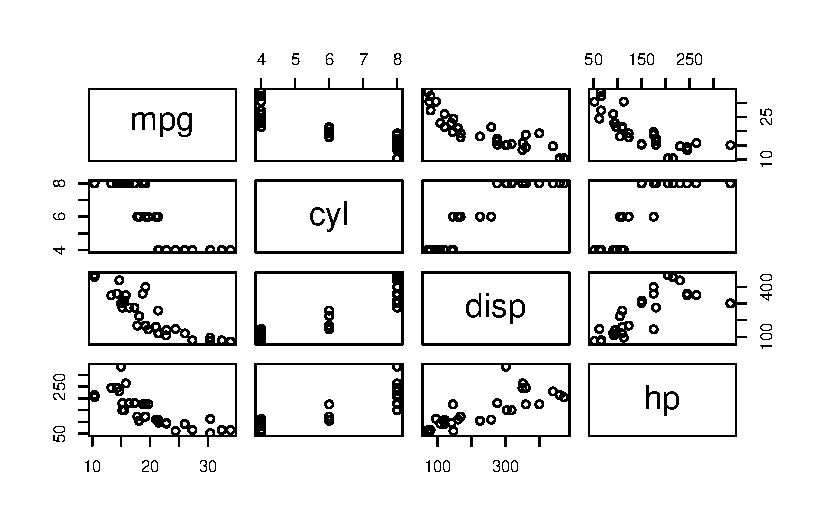
\includegraphics{./index_files/figure-pdf/fig-cars-1.pdf}

}

\end{figure}

This is Figura~\ref{fig-cars}.

See the Quarto manual for full examples and instructions.

\hypertarget{typesetting-mathematics}{%
\subsection{Typesetting mathematics}\label{typesetting-mathematics}}

If your thesis is going to contain heavy mathematical content, \LaTeX{}
will make it look beautiful, for HTML or PDF output.

The
\href{http://www.ctan.org/tex-archive/info/lshort/english/lshort.pdf}{Not
So Short Introduction to LaTeX} should tell you everything you need to
know for most cases of typesetting mathematics. If you need more
information, a much more thorough mathematical guide is available from
the AMS called,
\href{http://tug.ctan.org/info/short-math-guide/short-math-guide.pdf}{A
Short Math Guide to LaTeX}.

\hypertarget{in-closing}{%
\section{In Closing}\label{in-closing}}

Good luck and have lots of fun!

Guide written originally by

Sunil Patel: http://www.sunilpatel.co.uk\}\{www.sunilpatel.co.uk

and

Vel: http://www.LaTeXTemplates.com

and heavily shorted and adapted for \href{https://quarto.org/}{Quarto}
by \href{https://eeholmes.github.io}{Eli}.

\bookmarksetup{startatroot}

\hypertarget{sec-Chapter2}{%
\chapter{Chapter 2 Title}\label{sec-Chapter2}}

\hypertarget{main-section-1}{%
\section{Main Section 1}\label{main-section-1}}

Lorem ipsum dolor sit amet, consectetur adipiscing elit. Aliquam
ultricies lacinia euismod. Nam tempus risus in dolor rhoncus in interdum
enim tincidunt. Donec vel nunc neque. In condimentum ullamcorper quam
non consequat. Fusce sagittis tempor feugiat. Fusce magna erat, molestie
eu convallis ut, tempus sed arcu. Quisque molestie, ante a tincidunt
ullamcorper, sapien enim dignissim lacus, in semper nibh erat lobortis
purus. Integer dapibus ligula ac risus convallis pellentesque.

\hypertarget{subsection-1}{%
\subsection{Subsection 1}\label{subsection-1}}

Nunc posuere quam at lectus tristique eu ultrices augue venenatis.
Vestibulum ante ipsum primis in faucibus orci luctus et ultrices posuere
cubilia Curae; Aliquam erat volutpat. Vivamus sodales tortor eget quam
adipiscing in vulputate ante ullamcorper. Sed eros ante, lacinia et
sollicitudin et, aliquam sit amet augue. In hac habitasse platea
dictumst.

\hypertarget{subsection-2}{%
\subsection{Subsection 2}\label{subsection-2}}

Morbi rutrum odio eget arcu adipiscing sodales. Aenean et purus a est
pulvinar pellentesque. Cras in elit neque, quis varius elit. Phasellus
fringilla, nibh eu tempus venenatis, dolor elit posuere quam, quis
adipiscing urna leo nec orci. Sed nec nulla auctor odio aliquet
consequat. Ut nec nulla in ante ullamcorper aliquam at sed dolor.
Phasellus fermentum magna in augue gravida cursus. Cras sed pretium
lorem. Pellentesque eget ornare odio. Proin accumsan, massa viverra
cursus pharetra, ipsum nisi lobortis velit, a malesuada dolor lorem eu
neque.

\hypertarget{main-section-2}{%
\section{Main Section 2}\label{main-section-2}}

Sed ullamcorper quam eu nisl interdum at interdum enim egestas. Aliquam
placerat justo sed lectus lobortis ut porta nisl porttitor. Vestibulum
mi dolor, lacinia molestie gravida at, tempus vitae ligula. Donec eget
quam sapien, in viverra eros. Donec pellentesque justo a massa fringilla
non vestibulum metus vestibulum. Vestibulum in orci quis felis tempor
lacinia. Vivamus ornare ultrices facilisis. Ut hendrerit volutpat
vulputate. Morbi condimentum venenatis augue, id porta ipsum vulputate
in. Curabitur luctus tempus justo. Vestibulum risus lectus, adipiscing
nec condimentum quis, condimentum nec nisl. Aliquam dictum sagittis
velit sed iaculis. Morbi tristique augue sit amet nulla pulvinar id
facilisis ligula mollis. Nam elit libero, tincidunt ut aliquam at,
molestie in quam. Aenean rhoncus vehicula hendrerit.

\bookmarksetup{startatroot}

\hypertarget{sec-Chapter3}{%
\chapter{Chapter 3 Title}\label{sec-Chapter3}}

\begin{verbatim}
here() starts at D:/OneDrive - Universidad del Pacífico/quarto scripts/pucp-tesis
\end{verbatim}

This is an example of how to use this template to render journal
articles. This template is inspired by the Taylor and Francis rticles
template for rmarkdown, repurposed for the Quarto publishing system.

This quarto extension format supports PDF and HTML outputs. This
template is primarily focused on generating acceptable outputs from
Quarto, but renders an acceptable HTML output using the standard Quarto
options.

\hypertarget{quarto}{%
\section{Quarto}\label{quarto}}

Quarto enables you to weave together content and executable code into a
finished document. To learn more about Quarto see
\url{https://quarto.org}.

Here is a footnote reference,\footnote{Here is the footnote.} and
another.\footnote{Here's one with multiple blocks.}

\hypertarget{running-code}{%
\section{Running Code}\label{running-code}}

When you click the \textbf{Render} button a document will be generated
that includes both content and the output of embedded code. You can
embed code like this:

\begin{verbatim}
[1] 2
\end{verbatim}

This format hide chunks by default, but you can set \texttt{echo} option
to \texttt{true} locally in the chunk:

\begin{Shaded}
\begin{Highlighting}[]
\CommentTok{\# install.packages("broom")}
\CommentTok{\# install.packages("kableExtra")}
\FunctionTok{data}\NormalTok{(}\StringTok{"quine"}\NormalTok{, }\AttributeTok{package =} \StringTok{"MASS"}\NormalTok{)}
\NormalTok{m\_pois }\OtherTok{\textless{}{-}} \FunctionTok{glm}\NormalTok{(Days }\SpecialCharTok{\textasciitilde{}}\NormalTok{ (Eth }\SpecialCharTok{+}\NormalTok{ Sex }\SpecialCharTok{+}\NormalTok{ Age }\SpecialCharTok{+}\NormalTok{ Lrn)}\SpecialCharTok{\^{}}\DecValTok{2}\NormalTok{, }\AttributeTok{data =}\NormalTok{ quine, }\AttributeTok{family =}\NormalTok{ poisson)}
\NormalTok{kableExtra}\SpecialCharTok{::}\FunctionTok{kable\_styling}\NormalTok{(}
\NormalTok{  kableExtra}\SpecialCharTok{::}\FunctionTok{kbl}\NormalTok{(broom}\SpecialCharTok{::}\FunctionTok{tidy}\NormalTok{(m\_pois))}
\NormalTok{)}
\end{Highlighting}
\end{Shaded}

\hypertarget{tbl-glm}{}
\begin{table}
\caption{\label{tbl-glm}A table. }\tabularnewline

\centering
\begin{tabular}[t]{l|r|r|r|r}
\hline
term & estimate & std.error & statistic & p.value\\
\hline
(Intercept) & 2.9324591 & 0.0982638 & 29.8427305 & 0.0000000\\
\hline
EthN & -0.1739938 & 0.1213351 & -1.4339937 & 0.1515741\\
\hline
SexM & -0.7145197 & 0.1222943 & -5.8426235 & 0.0000000\\
\hline
AgeF1 & -0.0426993 & 0.1269111 & -0.3364507 & 0.7365310\\
\hline
AgeF2 & -0.0863239 & 0.1616403 & -0.5340495 & 0.5933073\\
\hline
AgeF3 & -0.1528978 & 0.1189753 & -1.2851227 & 0.1987494\\
\hline
LrnSL & 0.2160818 & 0.1455811 & 1.4842716 & 0.1377369\\
\hline
EthN:SexM & 0.4390243 & 0.0920790 & 4.7679077 & 0.0000019\\
\hline
EthN:AgeF1 & -0.9288934 & 0.1465738 & -6.3373786 & 0.0000000\\
\hline
EthN:AgeF2 & -1.3339773 & 0.1350383 & -9.8785113 & 0.0000000\\
\hline
EthN:AgeF3 & -0.1124246 & 0.1347842 & -0.8341080 & 0.4042202\\
\hline
EthN:LrnSL & 0.2641524 & 0.1137843 & 2.3215200 & 0.0202588\\
\hline
SexM:AgeF1 & -0.0556536 & 0.1630311 & -0.3413682 & 0.7328264\\
\hline
SexM:AgeF2 & 1.0994244 & 0.1528125 & 7.1945973 & 0.0000000\\
\hline
SexM:AgeF3 & 1.1594892 & 0.1385899 & 8.3663319 & 0.0000000\\
\hline
SexM:LrnSL & 0.0414270 & 0.1371756 & 0.3019998 & 0.7626522\\
\hline
AgeF1:LrnSL & -0.1301879 & 0.1568800 & -0.8298561 & 0.4066201\\
\hline
AgeF2:LrnSL & 0.3734020 & 0.1456293 & 2.5640585 & 0.0103456\\
\hline
AgeF3:LrnSL & NA & NA & NA & NA\\
\hline
\end{tabular}
\end{table}

\hypertarget{markdown-basics}{%
\section{Markdown Basics}\label{markdown-basics}}

This section of the template is adapted from
\href{https://quarto.org/docs/authoring/markdown-basics.html}{Quarto's
documentation on Markdown basics}.

\hypertarget{text-formatting}{%
\subsection{Text Formatting}\label{text-formatting}}

\begin{longtable}[]{@{}
  >{\raggedright\arraybackslash}p{(\columnwidth - 2\tabcolsep) * \real{0.5000}}
  >{\raggedright\arraybackslash}p{(\columnwidth - 2\tabcolsep) * \real{0.4444}}@{}}
\toprule()
\begin{minipage}[b]{\linewidth}\raggedright
Markdown Syntax
\end{minipage} & \begin{minipage}[b]{\linewidth}\raggedright
Output
\end{minipage} \\
\midrule()
\endhead
\begin{minipage}[t]{\linewidth}\raggedright
\begin{verbatim}
*italics* and **bold**
\end{verbatim}
\end{minipage} & \emph{italics} and \textbf{bold} \\
\begin{minipage}[t]{\linewidth}\raggedright
\begin{verbatim}
superscript^2^ / subscript~2~
\end{verbatim}
\end{minipage} & superscript\textsuperscript{2} /
subscript\textsubscript{2} \\
\begin{minipage}[t]{\linewidth}\raggedright
\begin{verbatim}
~~strikethrough~~
\end{verbatim}
\end{minipage} & \sout{strikethrough} \\
\begin{minipage}[t]{\linewidth}\raggedright
\begin{verbatim}
`verbatim code`
\end{verbatim}
\end{minipage} & \texttt{verbatim\ code} \\
\bottomrule()
\end{longtable}

\hypertarget{headings}{%
\subsection{Headings}\label{headings}}

\begin{longtable}[]{@{}
  >{\raggedright\arraybackslash}p{(\columnwidth - 2\tabcolsep) * \real{0.2639}}
  >{\raggedright\arraybackslash}p{(\columnwidth - 2\tabcolsep) * \real{0.4583}}@{}}
\toprule()
\begin{minipage}[b]{\linewidth}\raggedright
Markdown Syntax
\end{minipage} & \begin{minipage}[b]{\linewidth}\raggedright
Output
\end{minipage} \\
\midrule()
\endhead
\begin{minipage}[t]{\linewidth}\raggedright
\begin{verbatim}
## Header 2
\end{verbatim}
\end{minipage} & \begin{minipage}[t]{\linewidth}\raggedright
\hypertarget{header-2}{%
\section{Header 2}\label{header-2}}
\end{minipage} \\
\begin{minipage}[t]{\linewidth}\raggedright
\begin{verbatim}
### Header 3
\end{verbatim}
\end{minipage} & \begin{minipage}[t]{\linewidth}\raggedright
\hypertarget{header-3}{%
\subsection{Header 3}\label{header-3}}
\end{minipage} \\
\bottomrule()
\end{longtable}

\hypertarget{equations}{%
\subsection{Equations}\label{equations}}

Use \texttt{\$} delimiters for inline math and \texttt{\$\$} delimiters
for display math. For example:

\begin{longtable}[]{@{}
  >{\raggedright\arraybackslash}p{(\columnwidth - 2\tabcolsep) * \real{0.4444}}
  >{\raggedright\arraybackslash}p{(\columnwidth - 2\tabcolsep) * \real{0.3611}}@{}}
\toprule()
\begin{minipage}[b]{\linewidth}\raggedright
Markdown Syntax
\end{minipage} & \begin{minipage}[b]{\linewidth}\raggedright
Output
\end{minipage} \\
\midrule()
\endhead
\begin{minipage}[t]{\linewidth}\raggedright
\begin{verbatim}
inline math: $E = mc^{2}$
\end{verbatim}
\end{minipage} & inline math: \(E=mc^{2}\) \\
\begin{minipage}[t]{\linewidth}\raggedright
\begin{verbatim}
display math:

$$E = mc^{2}$$
\end{verbatim}
\end{minipage} & \begin{minipage}[t]{\linewidth}\raggedright
display math:\\
\[E = mc^{2}\]\strut
\end{minipage} \\
\bottomrule()
\end{longtable}

If assigned an ID, display math equations will be automatically
numbered:

\begin{equation}\protect\hypertarget{eq-black-scholes}{}{
\frac{\partial \mathrm C}{ \partial \mathrm t } + \frac{1}{2}\sigma^{2} \mathrm S^{2}
\frac{\partial^{2} \mathrm C}{\partial \mathrm C^2}
  + \mathrm r \mathrm S \frac{\partial \mathrm C}{\partial \mathrm S}\ =
  \mathrm r \mathrm C 
}\label{eq-black-scholes}\end{equation}

\hypertarget{other-blocks}{%
\subsection{Other Blocks}\label{other-blocks}}

\begin{longtable}[]{@{}
  >{\raggedright\arraybackslash}p{(\columnwidth - 2\tabcolsep) * \real{0.4167}}
  >{\raggedright\arraybackslash}p{(\columnwidth - 2\tabcolsep) * \real{0.3750}}@{}}
\toprule()
\begin{minipage}[b]{\linewidth}\raggedright
Markdown Syntax
\end{minipage} & \begin{minipage}[b]{\linewidth}\raggedright
Output
\end{minipage} \\
\midrule()
\endhead
\begin{minipage}[t]{\linewidth}\raggedright
\begin{verbatim}
> Blockquote
\end{verbatim}
\end{minipage} & \begin{minipage}[t]{\linewidth}\raggedright
\begin{quote}
Blockquote
\end{quote}
\end{minipage} \\
\begin{minipage}[t]{\linewidth}\raggedright
\begin{verbatim}
| Line Block
|   Spaces and newlines
|   are preserved
\end{verbatim}
\end{minipage} & \begin{minipage}[t]{\linewidth}\raggedright
Line Block\\
\hspace*{0.333em}\hspace*{0.333em}\hspace*{0.333em}Spaces and newlines\\
\hspace*{0.333em}\hspace*{0.333em}\hspace*{0.333em}are preserved
\end{minipage} \\
\bottomrule()
\end{longtable}

\hypertarget{sec-crf}{%
\subsection{Cross-references}\label{sec-crf}}

\begin{figure}

\caption{\label{fig-sunflower}Mi sunflower}

{\centering 
\includegraphics{Chapters/../Figures/Electron.pdf}

}

\end{figure}

\begin{longtable}[]{@{}
  >{\raggedright\arraybackslash}p{(\columnwidth - 2\tabcolsep) * \real{0.5278}}
  >{\raggedright\arraybackslash}p{(\columnwidth - 2\tabcolsep) * \real{0.4722}}@{}}
\toprule()
\begin{minipage}[b]{\linewidth}\raggedright
Markdown Format
\end{minipage} & \begin{minipage}[b]{\linewidth}\raggedright
Output
\end{minipage} \\
\midrule()
\endhead
\begin{minipage}[t]{\linewidth}\raggedright
\begin{verbatim}
@fig-sunflower is pretty.
\end{verbatim}
\end{minipage} & Figura~\ref{fig-sunflower} is pretty. \\
\begin{minipage}[t]{\linewidth}\raggedright
\begin{verbatim}
@tbl-glm was created from code.
\end{verbatim}
\end{minipage} & Tabla~\ref{tbl-glm} was created from code. \\
\begin{minipage}[t]{\linewidth}\raggedright
\begin{verbatim}
@sec-crf is this section.
\end{verbatim}
\end{minipage} & Sección~\ref{sec-crf} is this section. \\
\begin{minipage}[t]{\linewidth}\raggedright
\begin{verbatim}
@eq-black-scholes is above.
\end{verbatim}
\end{minipage} & Ecuación~\ref{eq-black-scholes} is above. \\
\bottomrule()
\end{longtable}

See the
\href{https://quarto.org/docs/authoring/cross-references.html}{Quarto
documentation on cross-references for more}.

\hypertarget{citations}{%
\section{Citations}\label{citations}}

This section of the template is adapted from the
\href{https://quarto.org/docs/authoring/footnotes-and-citations.html}{Quarto
citation documentation}.

Quarto supports bibliography files in a wide variety of formats
including BibTeX and CSL. Add a bibliography to your document using the
\texttt{bibliography} YAML metadata field. For example:

\begin{Shaded}
\begin{Highlighting}[]
\PreprocessorTok{{-}{-}{-}}
\FunctionTok{title}\KeywordTok{:}\AttributeTok{ }\StringTok{"My Document"}
\FunctionTok{bibliography}\KeywordTok{:}\AttributeTok{ references.bib}
\PreprocessorTok{{-}{-}{-}}
\end{Highlighting}
\end{Shaded}

See the \href{https://pandoc.org/MANUAL.html\#citations}{Pandoc
Citations} documentation for additional information on bibliography
formats.

\hypertarget{sec-citations}{%
\subsection{Citation Syntax}\label{sec-citations}}

Quarto uses the standard Pandoc markdown representation for citations.
Here are some examples:

\begin{longtable}[]{@{}
  >{\raggedright\arraybackslash}p{(\columnwidth - 2\tabcolsep) * \real{0.2929}}
  >{\raggedright\arraybackslash}p{(\columnwidth - 2\tabcolsep) * \real{0.7071}}@{}}
\toprule()
\begin{minipage}[b]{\linewidth}\raggedright
Markdown Format
\end{minipage} & \begin{minipage}[b]{\linewidth}\raggedright
Output
\end{minipage} \\
\midrule()
\endhead
\begin{minipage}[t]{\linewidth}\raggedright
\begin{verbatim}
Blah Blah [see
@knuth1984,
pp. 33-35;
also @wickham2015,
chap. 1]
\end{verbatim}
\end{minipage} & \begin{minipage}[t]{\linewidth}\raggedright
Blah Blah (see Knuth, 1984, pp. 33-35; also Wickham, 2015, chap.~1)
\end{minipage} \\
\begin{minipage}[t]{\linewidth}\raggedright
\begin{verbatim}
Blah Blah [@knuth1984,
pp. 33-35,
38-39 and passim]
\end{verbatim}
\end{minipage} & Blah Blah (Knuth, 1984, pp. 33-35, 38-39 and passim) \\
\begin{minipage}[t]{\linewidth}\raggedright
\begin{verbatim}
Blah Blah
[@wickham2015;
@knuth1984].
\end{verbatim}
\end{minipage} & Blah Blah (Knuth, 1984; Wickham, 2015). \\
\begin{minipage}[t]{\linewidth}\raggedright
\begin{verbatim}
Wickham says
blah
[-@wickham2015]
\end{verbatim}
\end{minipage} & Wickham says blah (2015) \\
\begin{minipage}[t]{\linewidth}\raggedright
\begin{verbatim}
@knuth1984
says blah.
\end{verbatim}
\end{minipage} & Knuth (1984) says blah. \\
\begin{minipage}[t]{\linewidth}\raggedright
\begin{verbatim}
@knuth1984 [p. 33]
says blah.
\end{verbatim}
\end{minipage} & Knuth (1984, p. 33) says blah. \\
\bottomrule()
\end{longtable}

See the \href{https://pandoc.org/MANUAL.html\#citations}{Pandoc
Citations} documentation for additional information on citation syntax.

To provide a custom citation stylesheet, provide a path to a CSL file
using the \texttt{csl} metadata field in your document, for example:

\begin{Shaded}
\begin{Highlighting}[]
\PreprocessorTok{{-}{-}{-}}
\FunctionTok{title}\KeywordTok{:}\AttributeTok{ }\StringTok{"My Document"}
\FunctionTok{bibliography}\KeywordTok{:}\AttributeTok{ references.bib}
\FunctionTok{csl}\KeywordTok{:}\AttributeTok{ nature.csl}
\PreprocessorTok{{-}{-}{-}}
\end{Highlighting}
\end{Shaded}

\newpage{}

Último texto.

\bookmarksetup{startatroot}

\hypertarget{referencias}{%
\chapter*{Referencias}\label{referencias}}
\addcontentsline{toc}{chapter}{Referencias}

\hypertarget{refs}{}
\begin{CSLReferences}{1}{0}
\leavevmode\vadjust pre{\hypertarget{ref-Reference3}{}}%
Arnold, A. S., Wilson, J. S., Boshier, M. G., \& Smith, J. (1998). A
Simple Extended-Cavity Diode Laser. \emph{Review of Scientific
Instruments}, \emph{69}(3), 1236-1239.
\url{http://link.aip.org/link/?RSI/69/1236/1}

\leavevmode\vadjust pre{\hypertarget{ref-Reference1}{}}%
Hawthorn, C. J., Weber, K. P., \& Scholten, R. E. (2001). Littrow
Configuration Tunable External Cavity Diode Laser with Fixed Direction
Output Beam. \emph{Review of Scientific Instruments}, \emph{72}(12),
4477-4479. \url{http://link.aip.org/link/?RSI/72/4477/1}

\leavevmode\vadjust pre{\hypertarget{ref-knuth1984}{}}%
Knuth, D. E. (1984). Literate programming. \emph{The Computer Journal},
\emph{27}(2), 97-111.

\leavevmode\vadjust pre{\hypertarget{ref-wickham2015}{}}%
Wickham, H. (2015). \emph{R Packages} (1st ed.). O'Reilly Media, Inc.

\leavevmode\vadjust pre{\hypertarget{ref-Reference2}{}}%
Wieman, C. E., \& Hollberg, L. (1991). Using Diode Lasers for Atomic
Physics. \emph{Review of Scientific Instruments}, \emph{62}(1), 1-20.
\url{http://link.aip.org/link/?RSI/62/1/1}

\end{CSLReferences}

\appendix
\addcontentsline{toc}{part}{Apéndices}

\hypertarget{sec-appA}{%
\chapter{Frequently Asked Questions}\label{sec-appA}}

\hypertarget{how-do-i-change-the-colors-of-links}{%
\section{How do I change the colors of
links?}\label{how-do-i-change-the-colors-of-links}}

Pass in \texttt{urlcolor:} in yaml. Or set these in the
include-in-header file.

\noindent If you want to completely hide the links, you can use:

\{\small\verb!\hypersetup{allcolors=.}!\}, or even better:

\{\small\verb!\hypersetup{hidelinks}!\}.

\noindent If you want to have obvious links in the PDF but not the
printed text, use:

\{\small\verb!\hypersetup{colorlinks=false}!\}.



\end{document}
